\documentclass[12pt]{article}
\usepackage{mathematics}
\newcommand{\Tl}{T_{\text{L}}}
\newcommand{\Tr}{T_{\text{R}}}

\begin{document}



\section{Urn}


\begin{mdframed}
  An urn contains a finite number of black and white balls. Balls are removed from the urn in a
  sequence of ``runs''. A run consists of selecting (uniformly at random) and removing from the urn
  one ball at a time until the first consecutive pair of different-colored balls is
  encountered. When this occurs, the second ball of the pair is replaced, and a new run is started.

  If the initial number of black and white balls are $(b, w)$, what is the probability that the
  final remaining ball is black?
\end{mdframed}


% \begin{claim*}
%   The probability if 50\% for all starting configurations in which there is at least one of
%   each. (This is consistent with the output of the recursive algorithm given below.)
% \end{claim*}


\begin{proof}~\\~\\
  Let $P_{b,w}$ be the probability that the last ball is black, starting with $b > 0$ black and
  $w > 0$ white balls.

  By direct enumeration of the possible sequences of events we know that
  \begin{align*}
    P_{1,1} &= 0.5\\
    P_{2,1} = P_{1,2} &= 0.5.
  \end{align*}

  Let the starting configuration be $(b, w)$ where $b, w > 0$.

  Let $X_i \in \{B, W\}$ be the color of the $i-th$ ball chosen.

  Suppose the first run consists of removing $b$ consecutive black balls. These are necessarily
  followed by a white ball (which is replaced), and then $w - 1$ more white balls, until one white
  ball remains. Thus the run looks like\\

  \begin{tabular}{|c|c|c|c|c|c|c|c|}
    $X_1$& $X_2$& $\ldots$& $X_b$& $X_{b+1}$& $X_{b+2}$& $\ldots$& $X_{b+w}$\\
    \hline
    $B$  & $B$  & $\ldots$& $B$  & $W$     & $W$     & $\ldots$& $W$\\
    $\frac{b}{b+w}$  & $$  & $\ldots$& $B$  & $W$     & $W$     & $\ldots$& $W$\\
  \end{tabular}

  The probability of this sequence of events is the product of

  \begin{tabular}{|c|c|c|c|c|c|c|c|}
    $X_1$& $X_2$    &                        $\ldots$& $X_b$              & $X_{b+1}$& $X_{b+2}$& $\ldots$& $X_{b+w}$\\
    \hline
    $B$             & $B$                  & $\ldots$& $B$                & $W$     & $W$     & $\ldots$& $W$\\
    $\frac{b}{b+w}$ & $\frac{b-1}{b-1+w}$  & $\ldots$& $\frac{1}{1 + w}$  & $1$     & $1$     & $\ldots$& $1$.
  \end{tabular}

  Alternatively, suppose the first run consists of removing $w$ consecutive white balls. These are
  necessarily followed by a black ball (which is replaced), and then $b - 1$ more black balls,
  until one black ball remains.

  The probability of this sequence of events is the product of

  \begin{tabular}{|c|c|c|c|c|c|c|c|}
    $X_1$& $X_2$    &                        $\ldots$& $X_w$              & $X_{1+w}$& $X_{2+w}$& $\ldots$& $X_{b+w}$\\
    \hline
    $W$             & $W$                  & $\ldots$& $W$                & $B$     & $B$     & $\ldots$& $B$\\
    $\frac{w}{b+w}$ & $\frac{w-1}{b+w-1}$  & $\ldots$& $\frac{1}{b + 1}$  & $1$     & $1$     & $\ldots$& $1$.
  \end{tabular}


\end{proof}








































% \subsection*{Ideas}
% \begin{enumerate}
% \item Note that $\Pr(\textup{last is black}) = \Pr(\textup{white goes extinct at some point})$.
% \item Work backwards from a minimal configuration. E.g. starting with $(\emptyset,1,1)$ we know the
%   probability is 50\%. This configuration could have been reached from two $n=2$ configurations:
%   \begin{enumerate}
%   \item $(W, 1, 1)$
%   \item $(B, 1, 1)$
%   \end{enumerate}

% \item Define a {\it configuration} to be (last-color-picked, current-n-black, current-n-white).\\
%   The initial configuration is $(\emptyset, b, w)$.\\
%   We can write transition probabilities like this:\\
%   \begin{tabular}{|c|c|c|c|}
%     \hline
%                          & $\emptyset, b, w$   & $B, b-1, w$        & $W, b, w-1$ \\
%     \hline
%                          &                     &                    &\\
%      $\emptyset, b, w$   & $0$                 & $\frac{b}{b + w}$  & $\frac{w}{b + w}$\\
%                          &                     &                    &\\
%     \hline
%                          &                     &                    &\\
%      $B,         b, w$   & $\frac{w}{b + w}$   & $0$                & $\frac{b}{b + w}$\\
%                          &                     &                    &\\
%     \hline
%                          &                     &                    &\\
%      $W,         b, w$   & $\frac{b}{b + w}$   & $\frac{w}{b + w}$  & $0$\\
%                          &                     &                    &\\
%     \hline
%   \end{tabular}
% \newpage
% \item We can calculate the probabilities via a recursive algorithm with memoization (``dynamic
%   programming''):

% \begin{minted}{python3}
% @memoized
% def P_last_is_black(b, w, prev=None):
%     """
%     Calculate probability that last removed ball is black.

%     b:    number of black balls
%     w:    number of white balls
%     prev: color of previously removed ball
%     """
%     if b == 0:
%         return 0.0
%     elif w == 0:
%         return 1.0
%     else:
%         # Probability conditional on removing black next
%         if prev == WHITE:
%             P_last_is_black_given_remove_black = P_last_is_black(b,     w, None)
%         else:
%             P_last_is_black_given_remove_black = P_last_is_black(b - 1, w, BLACK)

%         # Probability conditional on removing white next
%         if prev == BLACK:
%             P_last_is_black_given_remove_white = P_last_is_black(b,     w, None)
%         else:
%             P_last_is_black_given_remove_white = P_last_is_black(b, w - 1, WHITE)

%         P_remove_black = b / (b + w)
%         P_remove_white = 1 - P_remove_black

%         return (P_remove_black * P_last_is_black_given_remove_black +
%                 P_remove_white * P_last_is_black_given_remove_white)
% \end{minted}
% \end{enumerate}


\section{Points moving with constant velocity}

\let\x\undefined
\let\v\undefined
\let\A\undefined
\let\B\undefined
\let\|\undefined
\newcommand{\|}{\Big|\Big|}
\newcommand{\x}{\vec x}
\newcommand{\v}{\vec v}
\newcommand{\A}{\vec A}
\newcommand{\B}{\vec B}

\begin{mdframed}
  Let $\x_1(0), \ldots, \x_n(0) \in \R^2$ be known initial positions of $n$ particles. Each particle
  $\x_i$ is moving at constant velocity $\v_i$ so that $\x_i(t) = \x_i(0) + t\v_i$. For an unknown
  integer value $t^*$ the position of the particles spells a message in upper-case characters from
  the Latin alphabet. What is $t^*$? (And what is the message??)
\end{mdframed}

We hypothesize that the variance of the positions is at its minimum when $t=t^*$.

Let $\bar \v$ be the mean velocity and let $\bar \x(t)$ be the mean position of the points at time
$t$. Choose a coordinate system such that $\bar \x(0) = \0$. Therefore we have
\begin{align*}
  \bar \x(t) = \frac{1}{n}\sum_{\x=1}^n \x_i(t)
             = \bar \x(0) + t\bar \v
             = t\bar \v.
\end{align*}

Let $\sigma(t)$ be the variance of the points at time $t$:
\begin{align*}
  \sigma(t) &= \frac{1}{n}\sum_{i=1}^n\|\x_i(t) - \bar \x(t)\|^2\\
            &= \frac{1}{n}\sum_{i=1}^n\|\x_i(0) + t(\v_i - \bar \v)\|^2\\
            &= \frac{1}{n}\sum_{i=1}^n\sum_{j=1}^2\Big(x_{ij}(0) + t(v_{ij} - \bar v_j)\Big)^2.
\end{align*}
Therefore
\begin{align*}
  \sigma'(t) = \Bigg(\frac{1}{n}\sum_{i=1}^n\sum_{j=1}^22x_{ij}(0)(v_{ij} - \bar v_j)\Bigg) +
              2t\Bigg(\frac{1}{n}\sum_{i=1}^n\sum_{j=1}^2(v_{ij} - \bar v_j)^2\Bigg).
\end{align*}
Solving for $\sigma'(t) = 0$ gives
\begin{align*}
  t^* = \frac{-\sum_{i=1}^n\sum_{j=1}^2x_{ij}(0)(v_{ij} - \bar v_j)}
             {\sum_{i=1}^n\sum_{j=1}^2(v_{ij} - \bar v_j)^2}.
\end{align*}

\section{Repeated partial sum values}

\begin{mdframed}
  Let $a_1, a_2, \ldots, a_n$ be a finite real sequence, and define an infinite partial sum
  sequence, ``recycling'' the $a_i$:
  \begin{align*}
    (s_i) = a_1, a_1 + a_2, \ldots, \sum_{i=1}^na_i, \sum_{i=1}^na_i + a_1, \ldots.
  \end{align*}
  Does the partial sum sequence visit the same value twice and if so what is the first such value?
\end{mdframed}


\begin{proof}~\\
  First consider $n = 1$. Then $(s_i) = a_1, 2a_1, \ldots$ and there are repeats iff $a_1 = 0$.

  Next consider $n = 2$. Then $(s_i) = a_1, a_1 + a_2, 2a_1 + a_2, 2a_1 + 2a_2, \ldots$.
\end{proof}
\section{Tower struts}

\begin{mdframed}
  A tower of base width $w$ and height $h$ is composed of two sides inclined towards each other at
  the same angle $\beta$. A series of diagonal struts at angle $\alpha < \beta$ join the two
  sides. The two sides of the tower do not meet at the top.

  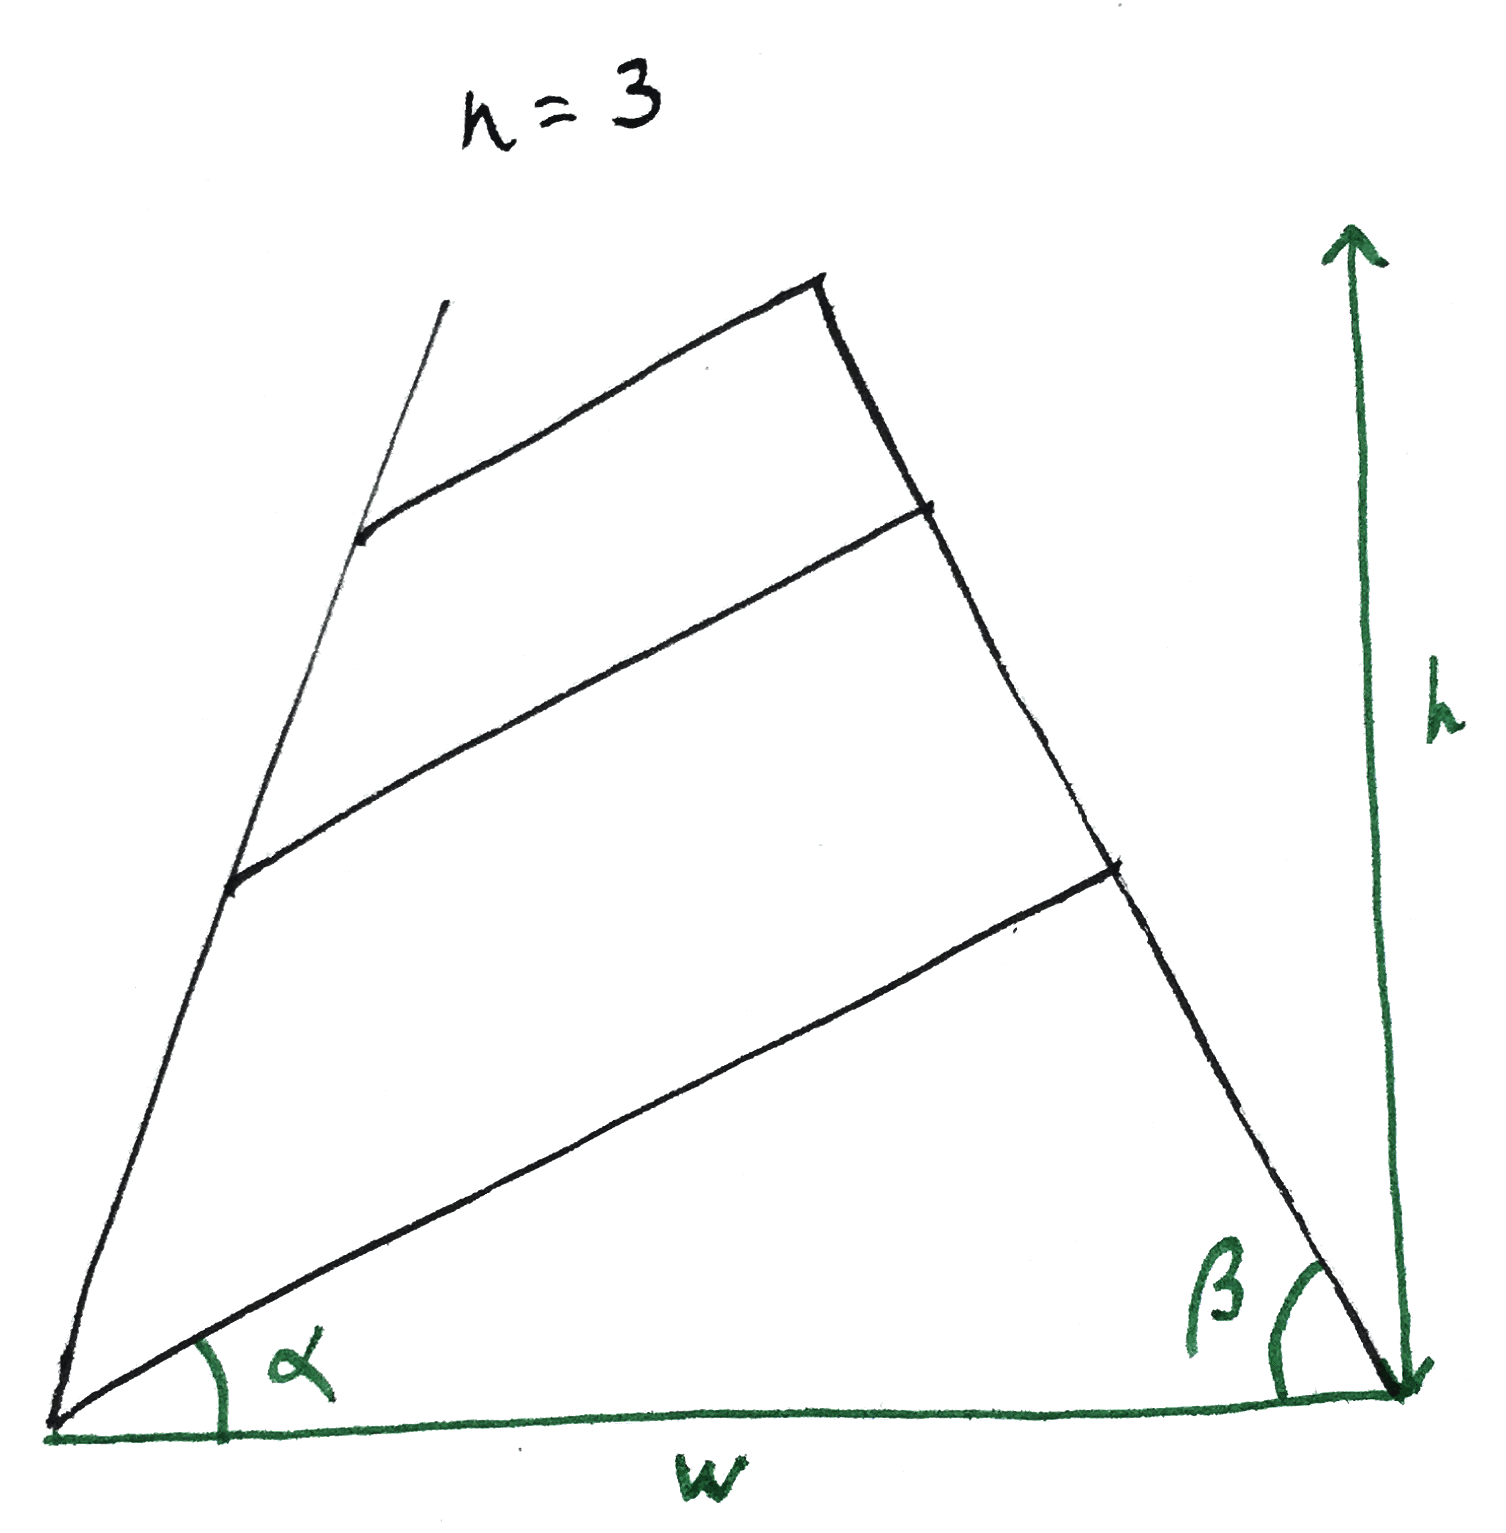
\includegraphics[width=200pt]{img/puzzles-tower-struts.png}

  There are $n$ diagonal struts, with the first strut starting at height 0 and the last strut
  ending at height $h$.

  $w, h, \beta$ and $n$ are given. What must $\alpha$ be?
\end{mdframed}
Note that the width of the base of the second storey is $w_2 = w - 2pw = (1 - 2p)w$.

Similarly, $w_3 = (1 - 2p)w_2 = (1 - 2p)^2w$.

So the final width is $w_{n+1} = (1 - 2p)^nw$.


Define the $n$-th storey to be the section of the tower containing the $n$-th strut.

Let $p = \frac{\tan\beta}{\tan\alpha + \tan\beta}$ be the ratio of the two angles.

The first strut intersects the right side at a horizontal distance $x = pw$ from the bottom right
hand corner (this can be proved by solving the equation $x\tan\beta = (w - x)\tan\alpha$, which
describes the height of intersection of the first strut with the right hand side).

Therefore the height of the first storey is $pw\tan\beta$.

Note that the width of the base of the second storey is $w - 2pw = (1 - 2p)w$.

Therefore the height of the second storey is $p(1 - 2p)w\tan\beta$, and the height of the $i$-th
storey is $p(1 - 2p)^{i-1}w\tan\beta$.

\newpage
% Therefore we need to find the $\alpha$ that solves $h = pw\tan\beta\sum_{i=0}^{n-1}(1 - 2p)^i$.

\begin{tabular}{l|l}
  $n$&$\frac{h}{w\tan\beta}$\\
  \hline\\
  $1$& $p$\\
  $2$& $p - 2p^2$\\
  $3$& $2p - 6p^2 + 4p^3$\\
  $4$& $3p - 12p^2 + 16p^3 - 8p^4$\\ \\
  $n$& $?$
\end{tabular}


$n = 1$
\begin{align*}
  \frac{h}{w\tan\beta}
  &= p
\end{align*}

$n = 2$
\begin{align*}
  \frac{h}{w\tan\beta}
  &= p(1 - 2p)\\
        &= p - 2p^2
\end{align*}

$n = 3$
\begin{align*}
  \frac{h}{w\tan\beta}
  &= p\Big((1 - 2p) + (1 - 2p)^2\Big)\\
  &= p(1 - 2p)(2 - 2p)\\
  &= (p - 2p^2)(2 - 2p)\\
  &= 2p - 6p^2 + 4p^3
\end{align*}

$n = 4$
\begin{align*}
  \frac{h}{w\tan\beta}
  &= p\Big((1 - 2p) + (1 - 2p)^2 + (1 - 2p)^3\Big)\\
  &= p\Big((1 - 2p)(2 - 2p) + (1 - 2p)^3\Big)\\
  &= p(1 - 2p)((2 - 2p) + (1 - 2p)^2)\\
  &= p(1 - 2p + 1 - 4p + 4p^2 + (1 - 2p)(1 - 4p + 4p^2))\\
  &= p(1 - 2p + 1 - 4p + 4p^2 + 1 - 4p + 4p^2 - 2p + 8p^2 - 8p^3)\\
  &= 3p - 12p^2 + 16p^3 - 8p^4\\
\end{align*}



\section{n-omino}
\begin{mdframed}
  You have a $n$-omino. (Like a tetris piece but with arbitrarily many pieces.)
  Now pick two points with uniform distribution on that piece. Prove that the
  probability that the line between them is contained on the piece is of the
  form $p - q\ln(r)$ where $p,q$ and $r$ are rational.
\end{mdframed}
~\\

Assumptions:
\begin{enumerate}
\item A random $n$-omino is generated as follows: place a square tile at an
  arbitrary location in a plane; while the number of tiles is less than $n$,
  choose an edge uniformly from among the available edges and place a tile
  adjoining that edge.
\end{enumerate}

Define an ``internal'' line to be a line connecting two points on an $n$-omino
that is contained in the $n$-omino.

Let $\omega$ denote the desired probability that a line between two points
chosen uniformly on an $n$-omino is internal.

For $n=1$ and $n=2$ we have $\omega = 1$, since the only possible
configurations are rectangles, and these are convex polygons.

For $n=3$ the configuration is a rectangle with probability $\frac{1}{3}$ and
an L-shape with probability $\frac{2}{3}$. In the former case the line is
always internal. In the latter case, if the first point is in the corner
square, then the line is always internal; otherwise, the probability that the
line is internal is equal to the
\begin{align*}
  \omega = \frac{1}{3}\cdot 1 + \frac{2}{3} \Big(\text{random area enclosed by line through center}\Big)
\end{align*}

\section{IMO}

\newpage
\begin{mdframed}
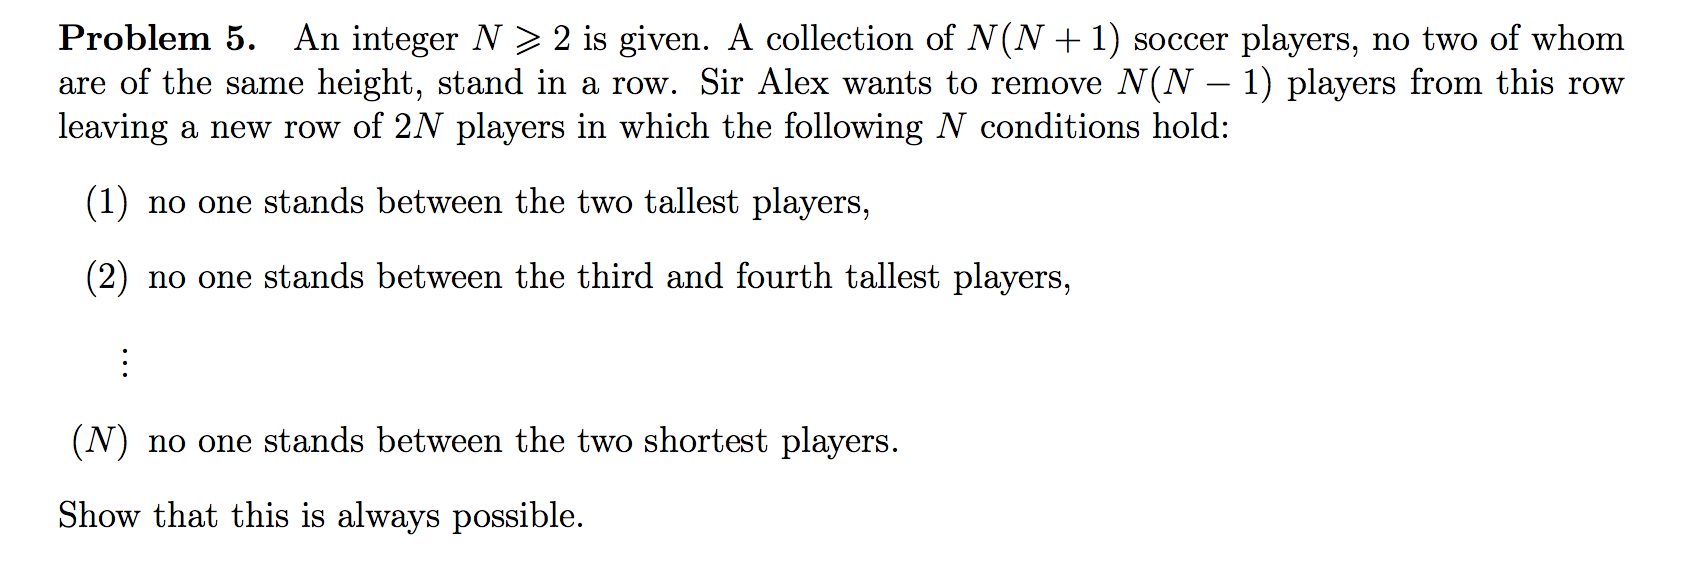
\includegraphics[width=400pt]{img/puzzles-imo-2017-5.png}
\end{mdframed}

\begin{enumerate}
\item Reverse direction: starting from a row of $2N$ satisfying the conditions, show that it is
  possible to generate an arbitrary superrow of $N(N+1)$ by inserting players?
\item Characterize the starting row as a permutation of $1, \ldots, N(N+1)$?

  Let $S_n$ be the set of permutations of $n$ objects.

  Let the starting row be $r \in S_{N(N+1)}$.

  Let $R_n \subset S_n$ be the subset of permutations of $n$ objects that satisfy the conditions.

  \begin{claim*}
    For all $\sigma \in S_{N(N+1)}$ there exists $\rho \in R_{2N}$ such that $\rho$ can be
    transformed into $\sigma$ via insertions.
  \end{claim*}

\item Formalize using a tuple of binary indicator variables $(e_1, e_2, \ldots, e_{N(N+1)})$, where
  $e_i \in \{0, 1\}$. Let $R_{N(N+1)}$ be the set of all possible starting rows and let $E_{N(N+1)}$
    be the set of all indicator tuples.

  Define the removal function
  $$f:R_{N(N+1)} \times E_{N(N+1)} \to R_{2N}$$
  and show for all $r \in R_{N(N+1)}$ there exists $e \in E_{N(N+1)}$ such that $f(r, e)$ satisfies
  the conditions?
\item Clearly the final number of players must be even, but what is the significance of the number
  $N(N+1)$?

\begin{verbatim}
|    |    <1 |     1 |     2 |     3 |     4 |
|----+-------+-------+-------+-------+-------|
| <1 | 12345 | 21345 | 23145 | 23415 | 23451 |
|  1 | 21345 | 12345 | 13245 | 13425 | 13452 |
|  2 | 31245 | 13245 | 12345 | 12435 | 12453 |
|  3 | 41235 | 14235 | 12435 | 12345 | 12354 |
|  4 | 51234 | 15234 | 12534 | 12354 | 12345 |
\end{verbatim}
\end{enumerate}

\newpage
\begin{mdframed}
   I pick ten points in the plane. I have ten coins.

   Show that I can cover all the points with the ten coins, with none of the coins overlapping.
\end{mdframed}

\begin{proof}
  Show (by identifying tiling region and using trigometry) that maximal packing of circles in plane
  covers just over $90\%$ of the plane.

  Therefore the expected number of points covered by exceeds 9.

  Therefore it is sometimes 10.
\end{proof}

\newpage
\section{Prisoners}
\begin{mdframed}
  There are 100 prisoners numbered 1 to 100. In a room there are 100 closed boxes. In each box
  there is a number between 1 and 100. Every box contains a different number. The prisoners enter
  the room one at a time. Once inside the room, the prisoner opens 50 boxes. If all prisoners
  encounter their own number then they all go free; otherwise they remain prisoners.
\end{mdframed}

Let $b_{ij}$ be the number of the $j$-th box chosen by prisoner $i$.

Represent the 50 boxes as 50 bits.

Thus $b_{ij} \in \{2^0, 2^1, 2^2, \ldots, 2^{99}\}$.

A selection of 50 boxes corresponds to an integer in $\{0, 1, 2, 3, \ldots, 2^{100} - 1\}$ which
has 50 bits set.

A selection $s$ contains box number $i$ if the binary representation of $s$ has the $i$-th bit set.

The prisoners are freed if and only if $s_1$

Does an optimal strategy have the property that every box is looked at by exactly 50 prisoners?

Divide prisoners into an odd and an even group. Then probability of being freed is $(1/2)^{50}$,
the same as each prisoner choosing a subset of boxes independently from all others.

\newpage
\section{Gas stations}

\begin{mdframed}
  There are $n$ gas stations at points $x_1, \ldots, x_n \in [0, 2\pi)$ of a circle.

  $2\pi$ units of gas are required to drive around the circle.

  The $i$-th gas station has $g_i$ units of gas, where $\sumin g_i = 2\pi$.

  Prove that there exists a gas station at which you can start, and make it around the circle
  without running out of gas.
\end{mdframed}

We assume, without loss of generality, that the $x_i$ are sorted in ascending order.

Any valid $\vec x$, $\vec g$ can be constructed as described below.

Make a cut in the circle at points $0, g_1, g_1 + g_2, \ldots, \sum_i^{n-1}g_i$.

The arcs thus defined represent the $g_i$, and their left endpoints represent the $x_i$.

Note that in this initial configuration the claim is true, since the arcs lie end-to-end with no
overlaps and cover the entire circle.

Take the left endpoint of the $g_1$ arc and drag it around the circle anticlockwise until it lies
at $x_1$. Shift the other arcs around to remove the overlap created.

Take the left endpoint of the $g_2$ arc and drag it around the circle anticlockwise until it lies
at $x_2$.

If this overlaps with $g_1$ then set $g_1 \leftarrow x_2, g_2 \leftarrow g_2 + (g_1 - x_2)$.

If this does not overlap with $g_1$... no not sure this leads to a proof.

\section{Hanging cable}

\begin{mdframed}
  A cable of length $L=80$m and uniform density hangs between two vertical poles of height
  $50$m. The lowest point of the cable is $20$m above the ground. How far apart are the poles?
\end{mdframed}

\subsection{Calculus of variations approach}

Let the density of the cable be $\rho$ kg/m. Introduce a coordinate system such that $x=0$ is the mid-point of
the cable, and $y = 0$ the height of the top of the poles. Let the distance between the poles be $2d$, so that
the poles are at $x = -d$ and $x = +d$. Let $y(x)$ be a function describing the shape of the cable.

The potential energy $V$ depends on the function $y$ describing the shape of the curve:
\begin{align*}
  V[y]
  &= \int_{-d}^d \sqrt{(\dx)^2 + (\dy)^2} \cdot \rho g y(x) \\
  &= \rho g \int_{-d}^d \sqrt{1 + y'(x)^2} \cdot y(x) \dx. \\
\end{align*}
Furthermore, we have two constraints. Firstly, the total length is $L = 80m$:
\begin{align*}
  \int_{-d}^d \sqrt{1 + y'(x)^2} \dx = L,
\end{align*}
and the endpoints are both at height zero: $y(-d) = y(d) = 0$.

To impose the total length constraint we use a Lagrange multiplier approach: this leads to reformulating the
problem as minimizing
\begin{align*}
  A[y] &= \int_{-d}^d \sqrt{1 + y'(x)^2} y(x) - \lambda \sqrt{1 + y'(x)^2} \dx \\
  &= \int_{-d}^d \(y(x) - \lambda\)\sqrt{1 + y'(x)^2} \dx. \\
\end{align*}
So this has the form $\int_{-d}^d f(y, y', x) \dx$, where $f(y, y', x) = \(y - \lambda\)\sqrt{1 + y'^2}$.
We have
\begin{align*}
  \pdfdyp =  (y - \lambda)(1 + y'^2)^{-1/2}y'
\end{align*}

and
 \begin{align*}
  \ddx \pdfdyp
  =& (y - \lambda) \cdot (1 + y'^2)^{-1/2}  \cdot y'' + \\
  & (y - \lambda)  \cdot \(\frac{-1}{2}\)(1 + y'^2)^{-3/2}2y'y'' \cdot y' + \\
  & y' \cdot (1 + y'^2)^{-1/2} \cdot y'.
\end{align*}
and
\begin{align*}
  \pdfdy = (1 + y'^2)^{1/2}.
\end{align*}

The Euler-Lagrange equations are
\begin{align*}
  \pdfdy = \ddx \pdfdyp.
\end{align*}
 \begin{align*}
  (1 + y'^2)^{1/2} =
  & (y - \lambda) \cdot (1 + y'^2)^{-1/2}  \cdot y'' + \\
  & (y - \lambda)  \cdot \(\frac{-1}{2}\)(1 + y'^2)^{-3/2}2y'y'' \cdot y' + \\
  & y' \cdot (1 + y'^2)^{-1/2} \cdot y'.
\end{align*}
 \begin{align*}
  (1 + y'^2) =
  & (y - \lambda)  y'' + \\
  & (y - \lambda) (-1)(1 + y'^2)^{-1}y'^2y'' + \\
  & y'^2.
\end{align*}
\begin{align*}
  1 = (y - \lambda)  y'' - (y - \lambda) (1 + y'^2)^{-1}y'^2y''
\end{align*}
\begin{align*}
 (y - \lambda) y''\(1 - \frac{y'^2}{1 + y'^2}\) - 1 = 0
\end{align*}

\begin{minted}{wolfram} :results latex
  el = (y[x] - lambda)y''[x](1 - y'[x]^2 / (1 + y'[x]^2)) - 1;
  DSolve[el == 0, y, x]
\end{minted}

\begin{align*}
\left\{\left\{y\to \left(\frac{1}{2} \left(-e^{-e^{c_1} x-2 c_1-e^{c_1} c_2}-e^{e^{c_1} x+e^{c_1} c_2}+2 \lambda \right)\right)\right\},\left\{y\to \left(\frac{1}{2} \left(-e^{-e^{c_1} x-e^{c_1} c_2}-e^{e^{c_1} x-2 c_1+e^{c_1} c_2}+2 \lambda \right)\right)\right\}\right\}
\end{align*}

Compare against doing it all in Mathematica. They seem to give the same result.

\begin{minted}{wolfram} :results latex
  (* hanging cable problem *)
  (* f = (y[x] - lambda)Sqrt[1 + y'[x]^2]; *)

  (* curve enclosing greatest area problem *)
  f = y[x] - lambda Sqrt[1 + y'[x]^2];

  pdfdy = D[f, y[x]];
  pdfdyp = D[f, y'[x]];
  ddxpdfdyp = D[pdfdyp, x];
  (* {pdfdy, pdfdyp, ddxpdfdyp, ddxpdfdyp - pdfdy} // Simplify *)
  (* ddxpdfdyp - pdfdy // Simplify *)
  DSolveValue[ddxpdfdyp == pdfdy, y, x]
\end{minted}

% DSolveValue::dsvb:
%    There are multiple solution branches for the equations, but DSolveValue
%     will return only one. Use DSolve to get all of the solution branches.

\begin{align*}
\{x\}\unicode{f4a1}\frac{1}{2} \left(-e^{-e^{c_1} x-2 c_1-e^{c_1} c_2}-e^{e^{c_1} x+e^{c_1} c_2}+2 \lambda \right)
\end{align*}

\begin{align*}
\text{DSolveExpr}\left(-\frac{(y(x)-\lambda ) y'(x)^2 y''(x)}{\left(y'(x)^2+1\right)^{3/2}}+\frac{(y(x)-\lambda ) y''(x)}{\sqrt{y'(x)^2+1}}+\frac{y'(x)^2}{\sqrt{y'(x)^2+1}}=\sqrt{y'(x)^2+1},y,x\right)
\end{align*}

\begin{align*}
\left\{\left\{y\to \left(\frac{1}{2} \left(-e^{-e^{c_1} x-2 c_1-e^{c_1} c_2}-e^{e^{c_1} x+e^{c_1} c_2}+2 \lambda \right)\right)\right\},\left\{y\to \left(\frac{1}{2} \left(-e^{-e^{c_1} x-e^{c_1} c_2}-e^{e^{c_1} x-2 c_1+e^{c_1} c_2}+2 \lambda \right)\right)\right\}\right\}
\end{align*}

\subsection{Initial attempts}
Consider the following approximation: the cable is divided into many straight line segments each of
length $\Delta L$. Segment $i$ is inclined at angle $\theta_i$ to the horizontal.

Let $\Delta x$ and $\Delta y$ be the horizontal and vertical displacements of segment $i$, so that
$\Delta L = \sqrt{(\Delta x)^2 + (\Delta y)^2}$. Cable density, and gravity, are constant and we
can ignore them by setting them equal to unity.

Restrict attention to segment $i$, and suppose that $\theta_i > 0$, i.e. this segment lies in the
right half of the curve.

\begin{mdframed}
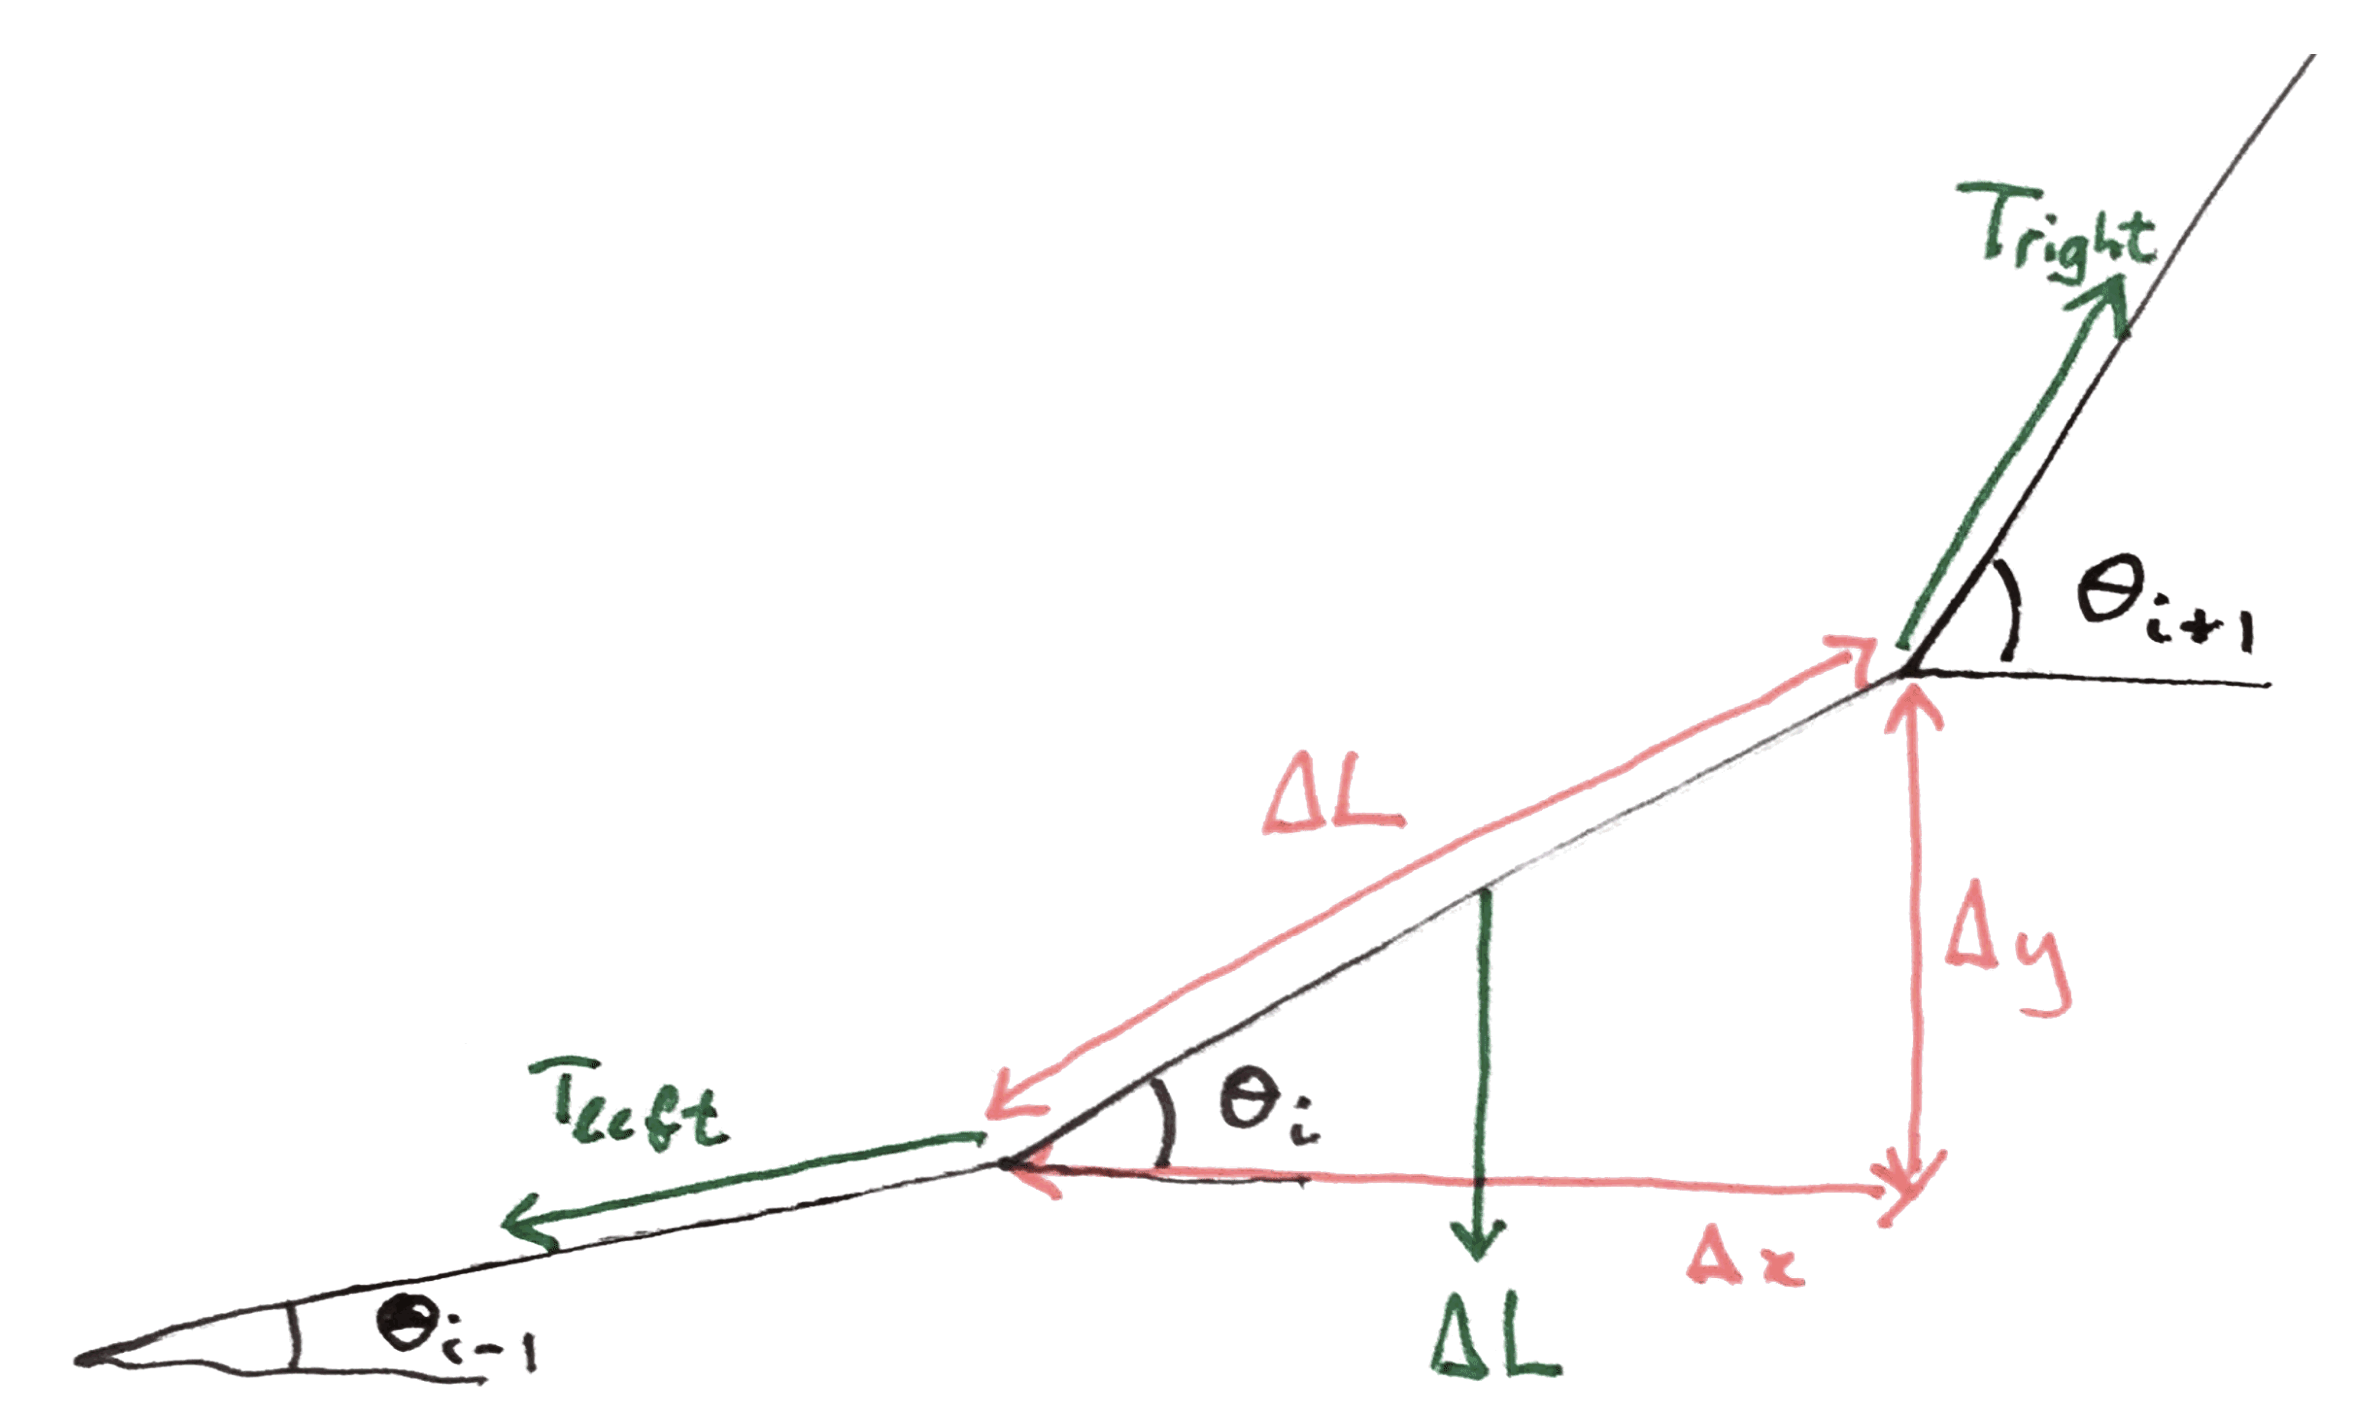
\includegraphics[width=300pt]{img/misc--puzzles--hanging-cable.png}
\end{mdframed}


Segment $i$ is subject to the following forces:
\begin{enumerate}
\item Weight $\Delta L$ acting vertically downwards.
\item Tension $T_l$ exerted by segment $i-1$ acting leftwards at angle $\theta_{i-1}$.
\item Tension $T_r$ exerted by segment $i+1$ acting rightwards at angle $\theta_{i+1}$.
\end{enumerate}
Consider the point where segment $i-1$ is attached to segment $i$. There are the following turning
moments around that point:
\begin{enumerate}
\item Clockwise $\frac{(\Delta L)^2}{2}\cos\theta_i$ due to the weight of segment $i$.
\item Clockwise $\Tr\cos\theta_{i+1}\Delta y$ due to the horizontal component of the tension force
  in segment $i+1$.
\item Anticlockwise $\Tr\sin\theta_{i+1}\Delta x$ due to the vertical component of the tension
  force in segment $i+1$.
\end{enumerate}

The segment is in equilibrium with respect to translational and rotational forces, giving the
following system of equations:

\begin{align*}
  \begin{cases}
    \Tl\cos\theta_{i-1} = \Tr\cos\theta_{i+1} ~~~~~~~&\text{no horizontal acceleration}\\
    \Tr\sin\theta_{i+1} = \Tl\sin\theta_{i-1} + \Delta L ~~~~~~~&\text{no vertical acceleration}\\
    \Tr\sin\theta_{i+1}\Delta x = \Tr\cos\theta_{i+1}\Delta y + \frac{(\Delta L)^2}{2}\cos\theta_i ~~~~~~~&\text{no turning moment.}\\
  \end{cases}
\end{align*}

\newpage

Number the segments starting with segment 0 being the rightmost segment, attached to the right
pole. We have the following system of equations:

\begin{align*}
  \begin{cases}
    T_0\cos\theta_0 = T_1\cos\theta_1                               ~~~~~~~&\text{no horizontal acceleration}\\
    T_1\sin\theta_1 + \Delta L = \frac{L}{2}                        ~~~~~~~&\text{no vertical acceleration}\\
    T_0\cos\theta_0\Delta y_0 +
    \frac{(\Delta L)^2}{2} \cos\theta_0 = T_0\sin\theta_0 \Delta x_0 ~~~~~~~&\text{no turning moment.}\\
  \end{cases}
\end{align*}


Let $H := T_i\cos\theta_i$, constant for all segments $i$.

Also, we have $T_i\sin\theta_i + i\Delta L = \frac{L}{2}$ for all $i$.

Therefore, substituting these into the turning moment equation, we have

\begin{align*}
  H\Delta y_0 + \frac{H(\Delta L)^2}{2T_0} &= \frac{L}{2} \Delta x_0 \\
  \Delta y_0 + \frac{(\Delta x_0)^2 + (\Delta y_0)^2}{2T_0} &= \frac{L}{2H} \Delta x_0.
\end{align*}


\newpage

Consider turning moments around the right attachment point:

\begin{align*}
  \frac{1}{2}(\Delta L)^2\cos\theta_0 + T_1\sin\theta_1\Delta L \cos\theta_0 &= T_1\cos\theta_1\Delta L \sin\theta_0\\
  \frac{1}{2}\Delta L + T_1\sin\theta_1 &= T_1\cos\theta_1 \tan\theta_0\\
  \frac{\Delta L}{2T_1\cos\theta_1} + \tan\theta_1 &= \tan\theta_0\\
  \tan\theta_1 &= \tan\theta_0 - \frac{\Delta L}{2H}\\
\end{align*}

Consider turning moments around the first articulation point:
\begin{align*}
  T_2\sin\theta_2\Delta L\cos\theta_1 + \frac{1}{2}(\Delta L)^2\cos\theta_1 &=
  T_2\cos\theta_2\Delta L\sin\theta_1 + \frac{1}{2}(\Delta L)^2\cos\theta_0\\
  T_2\sin\theta_2\cos\theta_1 + \frac{1}{2}\Delta L\cos\theta_1 &=
  T_2\cos\theta_2\sin\theta_1 + \frac{1}{2}\Delta L\cos\theta_0\\
  T_2\sin\theta_2 + \frac{1}{2}\Delta L &=
  H\tan\theta_1 + \frac{\Delta L\cos\theta_0}{2\cos\theta_1}\\
  \frac{L}{2} - 2\Delta L + \frac{1}{2}\Delta L &=
  H\tan\theta_1 + \frac{\Delta L\cos\theta_0}{2\cos\theta_1}\\
\end{align*}


\end{document}
